\documentclass{C://Aliases//Dropbox-MIT//Latex_Templates//personal}
\usepackage[utf8]{inputenc}
\usepackage[english]{babel}
\usepackage{epstopdf}

\usepackage[backend=biber, style=numeric, sorting=none]{biblatex}
\def\bibfont{\normalsize}

\addbibresource{jan-21-bib.bib}

\author{Jack Dinsmore}
\title{GCE UROP Summary}

\begin{document}
\maketitle

\begin{abstract}
We examine a millisecond pulsar model for the Galactic center excess and extract predictions for the total number of pulsars in the Galactic center, the number that can be resolved by \textit{Fermi} Gamma-Ray Space Telescope, and the fraction of resolvable luminosity for four luminosity functions found in the literature. We compare the latter two extracted values to observations. We perform the analysis for two models of the telescope's sensitivity: a step function probability of detection, and a more detailed, position-dependent model. Results depend strongly on the sensitivity model used, but no luminosity functions analyzed differed from the observables by more than a factor of ten.
\end{abstract}


\section{Introduction}
The Galactic Center GeV Excess (GCE) is an unexpected source of gamma radiation originating from with 20 degrees of the Galactic center, detected recently by the \textit{Fermi} Gamma-ray Space Telescope (\textit{Fermi}) \cite{Goodenough:2009gk, Eckner:2017oul}. Its origin is debated; the GCE holds potential to be the first evidence observed for dark matter annihilation \cite{Abazajian:2012pn,}, yet several studies have also shown that point sources such as millisecond pulsars (MSPs) may be responsible for the excess \cite{Wang:2005, Yuan:2014yda}.

The spacial distribution of the GCE has been found to match the square of a  Navarro-Frenk-White (NFW) profile with density $\rho_{\text{NFW}} = \parens{r / r_s}^{\gamma-1}\parens{1 + r/r_s}^{-3+\gamma}$, where $r_s \approx \SI{20}{\kilo\parsec}$ and $\gamma \approx 1.2$ \cite{Goodenough:2009gk, Zhong:2019ycb}. 

Previous work has interpreted this MSP model. Ref. \cite{Zhong:2019ycb} has proposed an exponentially damped power-law luminosity function
\begin{equation}
    \frac{dN}{dL} = L^{-\alpha} \expp{-\frac{L}{L_\text{max}}}\brackets{\Gamma\parens{1-\alpha, \frac{L_\text{min}}{L_\text{max}}}L_\text{max}^{1-\alpha}}^{-1},
    \label{eqn:power-law}
\end{equation}
restricting the range of luminosities to $[L_\text{min}, \infty)$, where $L_\text{min}$, $L_\text{max}$, and $\alpha$ are free parameters. This reference found that $(\SI{1e29}{\erg\per\second}, \SI{1e35}{\erg\per\second}, 1.94)$ is required reproduced observations. It assumed a step-function model of \textit{Fermi}'s sensitivity, where all the MSPs with luminosity $L>L_{th}$ are observed and those with $L<L_\text{th}$ are not, where the threshold luminosity was fixed at $L_\text{th}=\SI{e34}{\erg\per\second}$. They find that this model admits three million MSPs in the GCE, which differs from estimates based on the physical properties of observed MSPs that estimate the number of MSPs at the Galactic center at the order of 40,000 \cite{citation needed}.

Ref. \cite{osti_1305131} proposes a luminosity function of 
\begin{equation}
    \frac{dN}{dL} = \frac{\log_{10} e}{\sigma \sqrt{2\pi} L}\expp{-\frac{\parens{\log_{10} L - \log_{10} L_0}^2}{2\sigma^2}},
    \label{eqn:log-normal}
\end{equation}
where $L_0$ and $\sigma$ are free parameters. It fits this model to data from globular cluster data, yielding values $L_0 = \SI{8.8e33}{\erg\per\second}$ and $\sigma=0.62$. It predicts thousands of MSPs to occupy the GCE if the entire excess is to be explained by MSPs.

Ref. \cite{Ploeg:2020jeh} proposes several more intricate luminosity functions, derived from a model of the pulsars themselves. They find that the same model may be used for resolved, gobular cluster MSPs in the Galactic disk and unresolved MSPs at the Galactic center. We use their luminosity function generated for the galactic disk. It closely resembles a log-normal luminosity function as in equation \ref{eqn:log-normal}, where $L_0 = \SI{1.61e+32}{\erg\per\second}$ and $\sigma=0.700$. 

Finally, ref. \cite{Lee:2015fea} proposes a broken-power-law luminosity function of 
\begin{equation}
    \frac{dN}{dL} = \parens{\frac{\parens{1-n_1}\parens{1-n_2}}{L_b \parens{n_1 - n_2}}}\begin{cases}
        \parens{\fraci{L}{L_\text{b}}}^{-n_{1}} & L < L_{b} \\
        \parens{\fraci{L}{L_\text{b}}}^{-n_{2}} & L > L_b
    \end{cases}
    \label{eqn:nptf}
\end{equation}
where the free parameters  $n_1$, $n_2$, and $L_b$ were found via a Non-Poissonian Template Fitting model (NPTF) to be $(18.2, -0.66, \SI{8.66e+33}{\erg\per\second})$ for an NFW-squared-distributed population of MSPs named NFW PS. The paper proposes a second luminosity function named Disk PS with parameters $(17.5, 1.4, \SI{3.34e+35}{\erg\per\second})$, which is unnormalizable except when a minimum luminosity of pulsars $L_\text{min}$ is introduced. We set $L_\text{min}=\SI{1e29}{\erg\per\second}$, which is the same minimum pulsar luminosity used by ref. \cite{Zhong:2019ycb}. TThe turnover luminosity $L_\text{b}$ was given as a photon flux value in units of photons per centimeter squared per second; the process used to convert from photon flux to luminosity is detailed in the methods section.

All the above-mentioned luminosity functions are shown in figure \ref{fig:lum-funcs}.

\begin{figure}
    \centering
    \begin{subfigure}{.48\textwidth}
        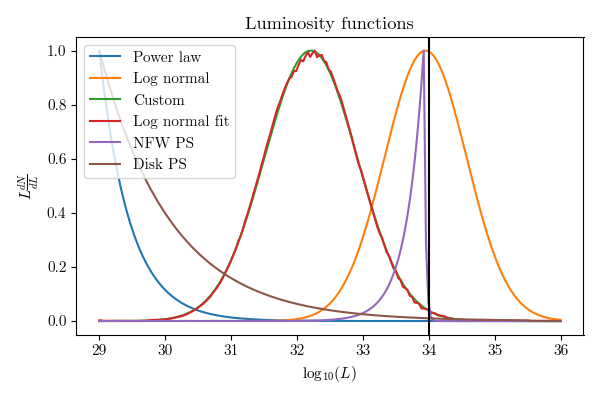
\includegraphics[width=\linewidth]{figs/superimposed.png}
        \caption{Luminosity functions as in the integral for expected number of MSPs.}
    \end{subfigure}
    \hfill
    \begin{subfigure}{.48\textwidth}
        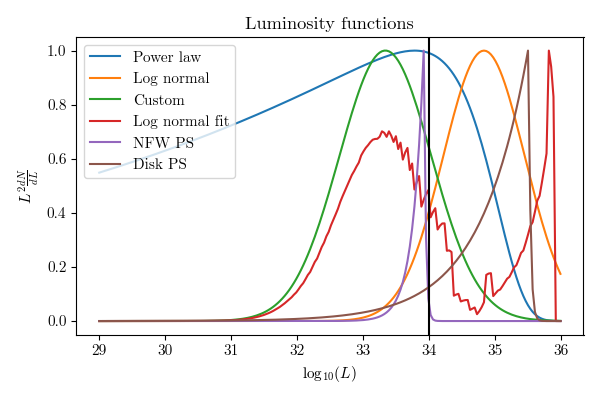
\includegraphics[width=\linewidth]{figs/superimposed-times-l.png}
        \caption{Luminosity functions, multiplied by L as in the integral for expected flux.}
    \end{subfigure}
    \caption{Luminosity functions considered in this summary. The black line indicates the threshold sensitivity used by ref. \cite{Zhong:2019ycb}.}
    \label{fig:lum-funcs}
\end{figure}

This UROP seeks to better understand the MSP model for the GCE by extracting the total number of MSPs in the GCE ($N$), the number resolvable with \textit{Fermi} ($N_\text{r}$), and the fraction of GCE luminosity emitted by resolved point sources ($R_\text{r}$). Observed values are $N_\text{r} \leq 47$ and $R_r \leq 0.2$ \cite{Zhong:2019ycb}.

For the purposes of this summary, we will take the GCE spectrum to be between $0.1$ and $100$ GeV, as in \cite{osti_1305131}. We take the total luminosity to be $L_\text{GCE}=\SI{6.756e+36}{\erg\per\second}$, which was obtained from ref. \cite{Zhong:2019ycb}'s value of $L_\text{GCE}=\SI{6.37e36}{\erg \per\second}$ for a range of 0.275 to 51.9 GeV, and extrapolating it using the power-law fit to the spectrum of the GCE produced in ref. \cite{Calore:2014xka}. 


\section{Methods}
We will use two models for \textit{Fermi}'s sensitivity to generate predictions of $N$, $N_\text{r}$, and $R_\text{r}$ for each luminosity model. The first is a step-function model like those used in \cite{Zhong:2019ycb, osti_1305131}, and the second is a more detailed, position-dependent model. For clarity, the region of interest of $2^\circ < |b| < 20^\circ$ and $|\ell| < 20^\circ$ will be denoted as $\mathcal{R}$.

For the first, step-function model, we assumed that all pulsars with luminosity $L < L_\text{th}$ were unresolvable, and all with $L>L_\text{th}$ were resolved, with threshold luminosity $L_\text{th} = \SI{e34}{\erg\per\second}$ as used in ref. \cite{Zhong:2019ycb}. A slightly higher value of $L_\text{th}$ may be more accurate, as shown by the flux distribution of resolved point sources obtained from the 4FGL data release \cite{Fermi-LAT:2019yla, Ballet:2020hze}. See fig. \ref{fig:observed-distros}. The expected luminosity they predict is
\begin{equation}
    L = N\int_{L_\text{min}}^{L_\text{max}} L P(L) dL.
\end{equation}
Here, the total number of pulsars in the GCE $N$ is set by requiring that $L = L_\text{GCE}$, where $L_\text{GCE} = \SI{6.756e36}{\erg\per\second}$ is the luminosity of the entire excess. The observed number of pulsars and their expected luminosity in this model are
\begin{equation}
    N_\text{r} = N\int_{L_\text{th}}^{L_\text{max}} P(L) dL
\end{equation}
\begin{equation}
    L_\text{r} = N \int_{L_\text{th}}^{L_\text{max}} L P(L) dL.
\end{equation}

\begin{figure}
    \centering
    \begin{subfigure}{.5\textwidth}
        \centering
        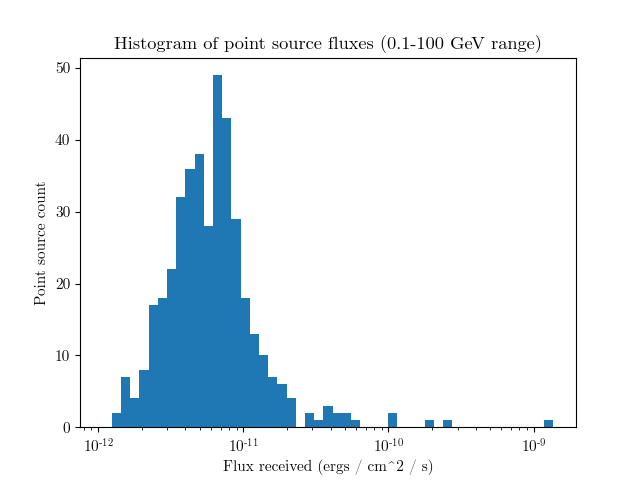
\includegraphics[width=.99\linewidth]{figs/flux-histo.png}
    \end{subfigure}%
    \begin{subfigure}{.5\textwidth}
        \centering
        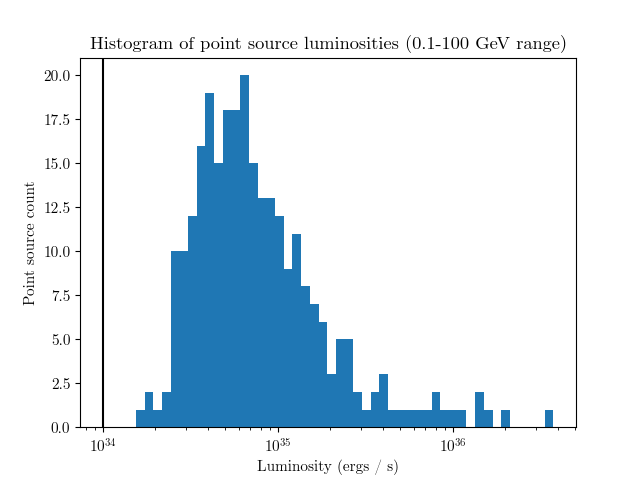
\includegraphics[width=.99\linewidth]{figs/luminosity-histo.png}
    \end{subfigure}
    \caption{\textit{Left}: Distribution of fluxes observed per resolved point source in the 4FGL catalog. \textit{Right}: Flux shown in \textit{Left} converted to luminosity, assuming that all the point sources are located at the galactic center at $r_\text{c} = \SI{8.5}{\kilo\parsec}$. The black line is the $L_\text{th}=\SI{1e34}{\erg\per\second}$ sensitivity threshold used in ref. \cite{Zhong:2019ycb}.}
    \label{fig:observed-distros}
\end{figure}

For the second, position-dependent sensitivity model, we obtained a map of position-dependent thresholds given as flux values from the same source \cite{Fermi-LAT:2019yla, Ballet:2020hze} (see figure \ref{fig:flux-thresholds}) and assumed that the MSPs are distributed according to the square of an NFW profile. Using an arbitrary normalized luminosity function $P(L)$, the total number of pulsars in the GCE is given by 
\begin{equation}
    N = \iint_{\mathcal{R}}\cos b dbd\ell \int_0^\infty s^2 ds A \rho_\text{NFW}^2 (r).
    \label{eqn:n}
\end{equation}
where the third integral is taken along the line of sight, with $r^2 = r_\text{c}^2 + s^2 - 2r_\text{c} s \cos b \cos \ell$, where $r_\text{c} = \SI{8.5}{\kilo\parsec}$ is the distance to the galactic center. Here, $A$ is the constant of proportionality of $\rho_{NFW}^2$, which is fixed by setting the total flux of the GCE
\begin{equation}
    F = \iint_{\mathcal{R}}\cos b dbd\ell \int_0^\infty s^2 ds A \rho_{NFW}^2 (r) \frac{1}{4\pi s^2}\int_{L_{min}}^{L_{max}}LP(L)dL.
    \label{eqn:f}
\end{equation}
equal to the observed value $F_\text{GCE}$. Then the number of resolved MSPs and resolved flux can be calculated respectively as 
\begin{equation}
    N_r = \iint_{\mathcal{R}}\cos b dbd\ell \int_0^\infty s^2 ds A \rho_\text{NFW}^2 (r) \int_{L_\text{th}(b, \ell)}^{L_\text{max}}P(L)dL.
    \label{eqn:nr}
\end{equation}
\begin{equation}
    F_r = \iint_{\mathcal{R}}\cos b dbd\ell \int_0^\infty s^2 ds A \rho_\text{NFW}^2 (r) \frac{1}{4\pi s^2}\int_{L_\text{th}(b, \ell)}^{L_\text{max}}LP(L)dL.
    \label{eqn:fr}
\end{equation}
with the ratio of resolved flux to total flux being $R_\text{r} = F_\text{r}/F$. Note that $L_\text{th}$ in the above equations was given by $L_\text{th}(b, \ell) = 4\pi s^2 F_\text{th}(b, \ell)$, where $F_\text{th}(b, \ell)$ was given in the sensitivity map (figure \ref{fig:flux-thresholds}).

\begin{figure}
    \centering
    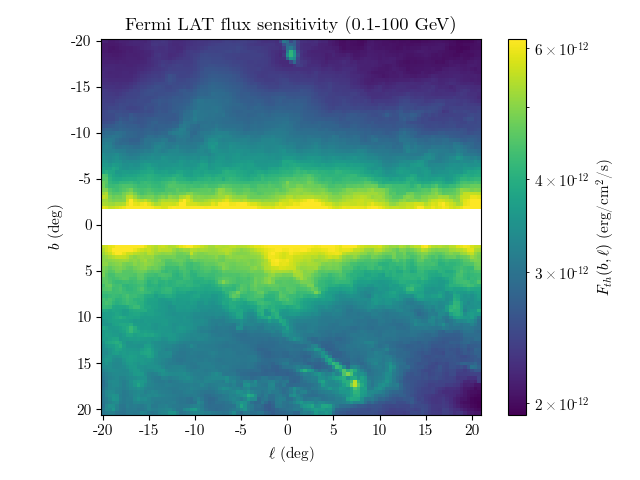
\includegraphics[width=.6\linewidth]{figs/flux-thresholds.png}
    \caption{Position-dependent flux values per point source necessary in order to resolve the point source. A GCE location of $2^\circ < |b| < 20^\circ$, $|\ell| < 20^\circ$ is shown.}
    \label{fig:flux-thresholds}
\end{figure}

We calculated the observed flux of the GCE $F_\text{GCE}$ from the observed luminosity $L_\text{GCE}$ by assuming an NFW-distributed population of $N$ MSPs, all with the same luminosity $L = L_\text{GCE} / N$, yielding a flux of 
\begin{equation}
    F_\text{GCE} = \frac{L_\text{GCE}}{4\pi}\brackets{\iint_{\mathcal{R}}\cos b db d\ell \int_0^\infty ds \rho_\text{NFW}^2 (r)}\brackets{\iint_{\mathcal{R}}\cos b db d\ell \int_0^\infty s^2 ds \rho_\text{NFW}^2 (r)}^{-1}
    \label{eqn:l-to-f}
\end{equation}
via equations \ref{eqn:n} and \ref{eqn:f}. The calculated value was $F_\text{GCE}=\SI{7.631e-10}{\erg\per\centi\meter\squared\per\second}$, which differs from the naive value of $F_\text{GCE} = L_\text{GCE} / (4\pi r_c^2)$ by 4.2\%.

The step function sensitivity model can be conveniently thought of as a simplified version of the position-dependent model, where $L_\text{th}(b, \ell)$ has been set to a constant value of $L_\text{th}$ throughout the region of interest, and the division by $4\pi s^2$ of equations \ref{eqn:f} and \ref{eqn:fr} has been approximated by the constant value of $4\pi r_\text{c}^2$.
%%%%%%%%%%%% ADDRESS THE COMMENT

The luminosity function given in ref. \cite{Lee:2015fea} gave the turnover luminosity $L_b$ as a flux value of $F_{\gamma, \text{b}}$ in units of photons per centimeter squared per second, which we convert to an energy flux value by $F_\text{b} = E_\gamma F_{\gamma, \text{b}}$ with an average energy per photon of
\begin{equation}
    E_\gamma = \brackets{\int_{\SI{1.893}{\giga\electronvolt}}^{\SI{11.943}{\giga\electronvolt}} \frac{dN_\gamma}{dE} E dE} \brackets{\int_{\SI{1.893}{\giga\electronvolt}}^{\SI{11.943}{\giga\electronvolt}} \frac{dN_\gamma}{dE} E dE }^{-1},
    \label{eqn:photon-energy}
\end{equation}
where $\fraci{dN_\gamma}{dE} = A E^{-\alpha} \expp{-E / E_\text{cut}}$ is the photon spectrum of the GCE given by ref. \cite{Calore:2014xka}, with $\alpha \approx 2.25$ and $E_\text{cut} = \SI{2.25}{\giga\electronvolt}$. The range of integration of equation \ref{eqn:photon-energy} was set by the GCE spectrum range used in  ref. \cite{Lee:2015fea}. The proportionality constant is fixed by assertion that the (known) total observed flux of the GCE in the $0.1-100$ GeV is $F_\text{GCE} = \int_{\SI{0.1}{\giga\electronvolt}}^{\SI{100}{\giga\electronvolt}} \parens{\fraci{dN_\gamma}{dE}}E dE$. The turnover luminosity was then calculated using the flux-luminosity ratio given in equation \ref{eqn:l-to-f}.


\section{Results}
For each of the luminosity functions described above, we calculated $N$, $N_r$, and $R_r = F_r / F$ using both the step-function sensitivity model and the position-dependent model. Results are displayed in table \ref{tab:point-results}.

Since the power-law and log-normal luminosity function models form a two-dimensional space of functions, parameterized by $(L_\text{min}, L_\text{max})$ and $(L_0, \sigma)$ respectively (we keep $\alpha =1.94$ for the power-law), we may display the predicted number of pulsars for all configurations, and superimpose the two observational constraints: $N_\text{r} = 47$ and $R_\text{r} = 0.2$. This is done using the step-function sensitivity model and the position-dependent sensitivity model in figure \ref{fig:contours}.

For the position-dependent sensitivity, we can easily simulate the power of a more advanced, next-generation gamma ray telescope by dividing the sensitivity per pixel provided by refs \cite{Fermi-LAT:2019yla, Ballet:2020hze} by some position-independent constant. This was done for a 2-, 5-, and 10-times improvement in sensitivity for both the power-law and the log-normal luminosity functions, and is shown in figure \ref{fig:sensitivity-increase}.

\begin{figure}
    \centering
    \begin{subfigure}[t]{\textwidth}
        \centering
        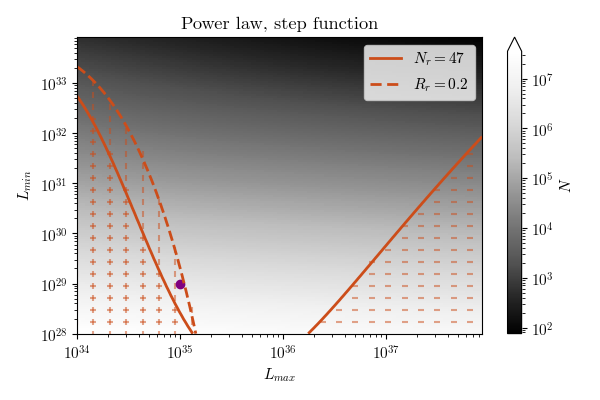
\includegraphics[width=.48\linewidth]{figs/power-law/power-law-step.png}
        \hfill
        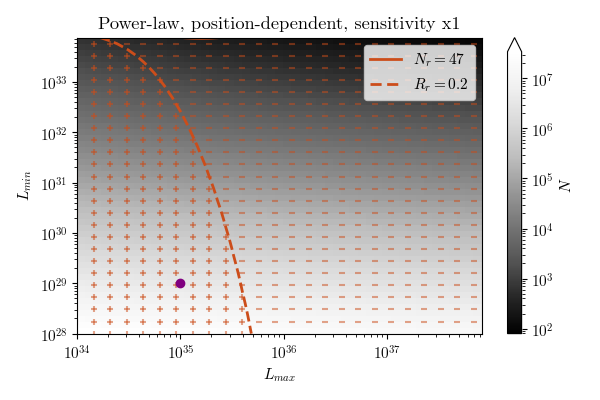
\includegraphics[width=.48\linewidth]{figs/power-law/power-law-pos-x1.png}
        \caption{Power law luminosity functions. The purple point is the configuration identified in ref. \cite{Zhong:2019ycb}: $L_\text{min}=\SI{1e29}{\erg\per\second}$, $L_\text{max} = \SI{1e35}{\erg\per\second}$.}
        \label{fig:power-law-contours-step}
    \end{subfigure}%
    \hfill
    \begin{subfigure}[t]{\textwidth}
        \centering
        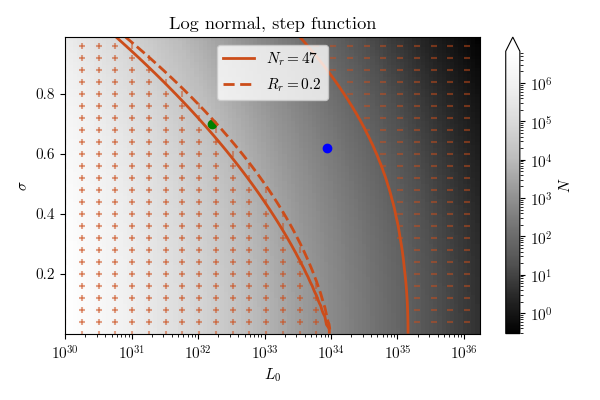
\includegraphics[width=.48\linewidth]{figs/log-normal/log-normal-step.png}
        \hfill
        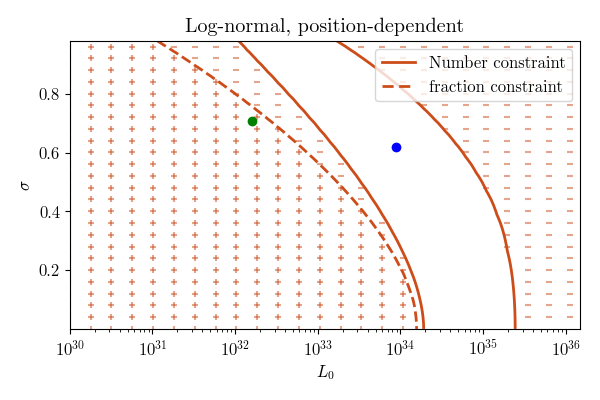
\includegraphics[width=.48\linewidth]{figs/log-normal/log-normal-pos-x1.png}
        \caption{Log normal luminosity functions. The blue point is the configuration identified in ref. \cite{osti_1305131}: $L_0=\SI{8.8e33}{\erg\per\second}$, $\sigma=0.62$, and the green point is a fit to the luminosity function found in ref. \cite{Ploeg:2020jeh}: $L_0=\SI{1.61e32}{\erg\per\second}$, $\sigma=0.700$.}
    \end{subfigure}
    \caption{Predicted number of MSPs $N$ plotted for different configurations of luminosity functions, with the $N_\text{r}=47$ constraint and the $R_\text{r}=0.2$ constraint  superimposed. \textit{Left}: The step-function sensitivity model was used, with $L_\text{th} = \SI{e34}{\erg\per\second}$. \textit{Right}: The position-depeondent sensitivity model was used. The \texttt{-} shading represents configurations that satisfy the number constraint $N_\text{r} < 47$, while the \texttt{|} shading represents those with $R_r < 0.2$. The \texttt{+} shading represents both.}
    \label{fig:contours}
\end{figure}



\begin{figure}
    \centering
    \begin{subfigure}[t]{.45\textwidth}
        \centering
        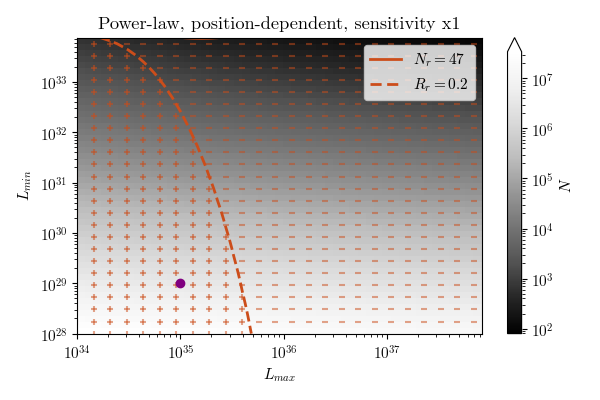
\includegraphics[width=.99\linewidth]{figs/power-law/power-law-pos-x1.png}
        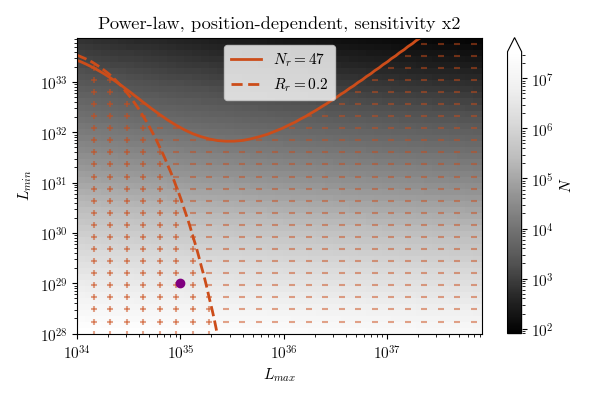
\includegraphics[width=.99\linewidth]{figs/power-law/power-law-pos-x2.png}
        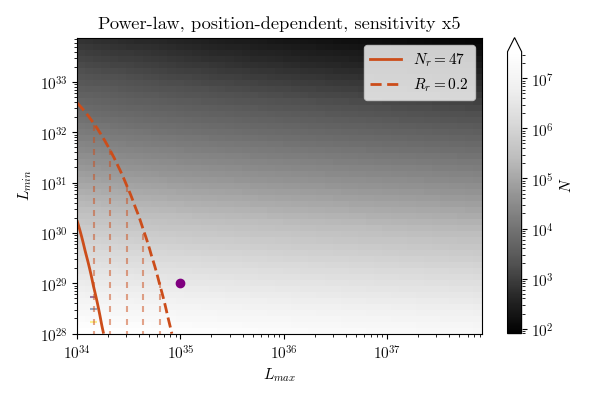
\includegraphics[width=.99\linewidth]{figs/power-law/power-law-pos-x5.png}
        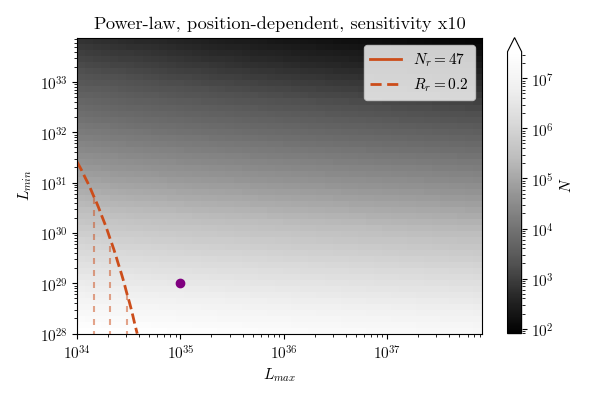
\includegraphics[width=.99\linewidth]{figs/power-law/power-law-pos-x10.png}
        \caption{Power law luminosity functions}
    \end{subfigure}%
    \hfill
    \begin{subfigure}[t]{.45\textwidth}
        \centering
        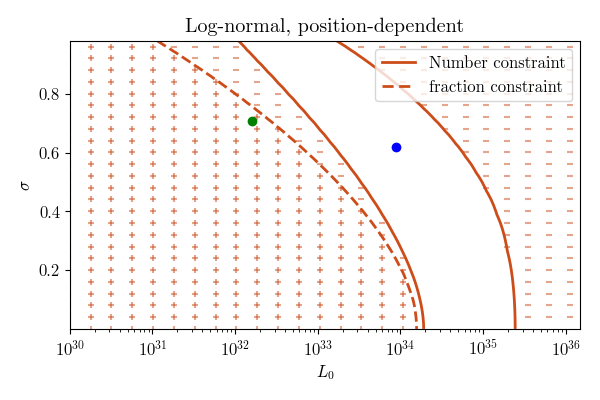
\includegraphics[width=.99\linewidth]{figs/log-normal/log-normal-pos-x1.png}
        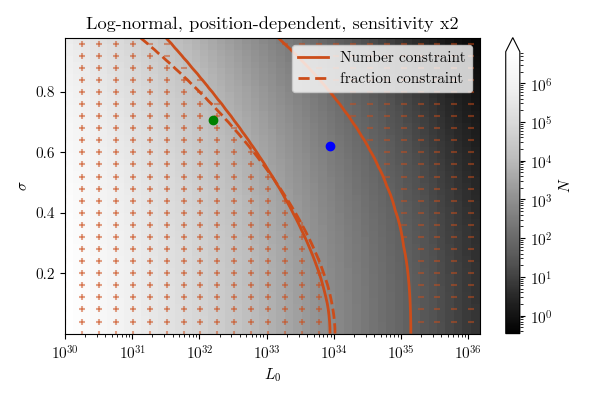
\includegraphics[width=.99\linewidth]{figs/log-normal/log-normal-pos-x2.png}
        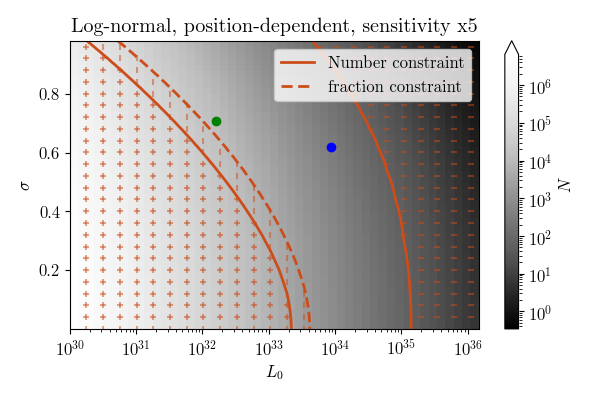
\includegraphics[width=.99\linewidth]{figs/log-normal/log-normal-pos-x5.png}
        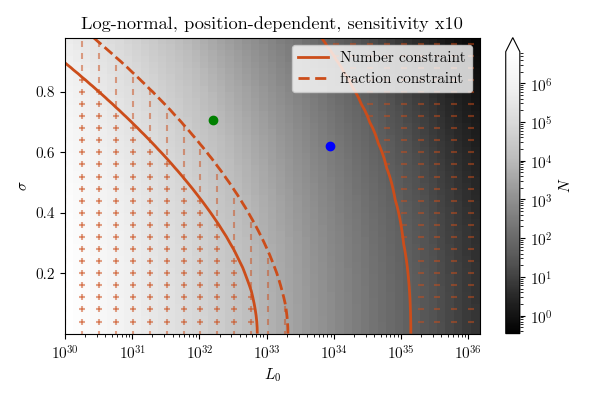
\includegraphics[width=.99\linewidth]{figs/log-normal/log-normal-pos-x10.png}
        \caption{Log normal luminosity functions}
    \end{subfigure}
    \caption{Predicted number of MSPs over the space of power-law and log-normal luminosity functions, and different sensitivities of the telescope, with current observational constraints superimposed.}
    \label{fig:sensitivity-increase}
\end{figure}

Using the position-dependent sensitivity model, the predicted number of pulsars is largely unchanged as expected, but the observational constraints differ greatly from the step-function sensitivity model.

\begin{table}
    \centering
    \begin{subtable}[h]{0.9\textwidth}
        \centering
        \begin{tabular}{|l|c|c|c|}
            \hline
            Luminosity function & $N$ & $N_r$ & $R_r$ \\ \hline
            Observations & - & 47 & 0.2 \\
            Ref. \cite{Zhong:2019ycb}: Power-law & $\num{3.54e6}$ & 50.0 & 0.193 \\
            Ref. \cite{osti_1305131}: Log-normal & 277 & 129 & 0.910 \\
            Ref. \cite{Ploeg:2020jeh}: Custom  & $\num{8.76e3}$ & 54.5 & 0.355 \\
            Ref. \cite{Ploeg:2020jeh}: Log-normal fit  & $\num{1.14e4}$ & 59.7 & 0.171 \\
            Ref. \cite{Lee:2015fea}: Broken power-law, NFW PS & $\num{1.23e3}$ & 4.41 & $\num{6.94e-3}$ \\
            Ref. \cite{Lee:2015fea}: Broken power-law, Disk PS & $\num{1.21e4}$ & 92.1 & 0.880 \\ \hline
        \end{tabular}
        \caption{Results for a step-function sensitivity model with $L_{th} = \SI{e34}{\erg\per\second}$}
        \label{tab:step}
    \end{subtable}

    \vspace{1em}

    \begin{subtable}[h]{0.9\textwidth}
        \centering
        \begin{tabular}{|l|c|c|c|}
            \hline
            Luminosity function & $N$ & $N_\text{r}$ & $R_\text{r}$ \\ \hline
            Observations & - & 47 & 0.2 \\
            Ref. \cite{Zhong:2019ycb}: Power-law & $\num{3.42e6}$ & 10.2 & 0.101 \\
            Ref. \cite{osti_1305131}: Log-normal & 268 & 44.8 & 0.692 \\
            Ref. \cite{Ploeg:2020jeh}: Custom  & $\num{8.48e3}$ & 9.66 & 0.266 \\
            Ref. \cite{Ploeg:2020jeh}: Log-normal fit  & $\num{1.11e4}$ & 7.76 & 0.0648 \\
            Ref. \cite{Lee:2015fea}: Broken power-law, NFW PS & $\num{1.19e3}$ & 4.06 & 0.0283 \\
            Ref. \cite{Lee:2015fea}: Broken power-law, Disk PS & $\num{1.17e4}$ & 42.1 & 0.751 \\ \hline
        \end{tabular}
        \caption{Results for a position-dependent sensitivity function}
        \label{tab:position}
    \end{subtable}
    \caption{Predictions for $N$, the total number of MSPs required to make up the GCE; $N_\text{r}$, the number of resolvable MSPs; and $R_\text{r}$, the fraction of luminosity that comes from resolved sources. The luminosity functions used are those proposed by the various references cited. For the final luminosity function, a cutoff value of $L_\text{min}=\SI{1e29}{\erg\per\second}$ was used so that the function would be normalizable. The observed values are discussed in ref. \cite{Zhong:2019ycb}.}
    \label{tab:point-results}
\end{table}
\begin{table}
    \centering
    \begin{subtable}[h]{0.9\textwidth}
        \centering
        \begin{tabular}{|l|c|c|c|c|}
            \hline
            Luminosity function & $\times 1$ & $\times 2$ & $\times 5$ & $\times 10$ \\ \hline
            Ref. \cite{Zhong:2019ycb}: Power-law & 10.2 & 26.5 & 79.1 & 167 \\
            Ref. \cite{osti_1305131}: Log-normal & 44.8 & 82.1 & 145 & 191 \\
            Ref. \cite{Ploeg:2020jeh}: Custom  & 9.66 & 26.1 & 110 & 281 \\
            Ref. \cite{Ploeg:2020jeh}: Log-normal fit  & 7.76 & 28.3 & 128 & 343 \\
            Ref. \cite{Lee:2015fea}: Broken power-law, NFW PS & 4.06 & 27.1 & 318 & 819 \\
            Ref. \cite{Lee:2015fea}: Broken power-law, Disk PS & 42.1 & 64.7 & 106 & 149 \\ \hline
        \end{tabular}
        \caption{$N_r$ values for different sensitivities.}
    \end{subtable}

    \vspace{1em}

    \begin{subtable}[h]{0.9\textwidth}
        \centering
        \begin{tabular}{|l|c|c|c|c|}
            \hline
            Luminosity function & $\times 1$ & $\times 2$ & $\times 5$ & $\times 10$ \\ \hline
            Ref. \cite{Zhong:2019ycb}: Power-law & 0.101 & 0.157 & 0.237 & 0.298 \\
            Ref. \cite{osti_1305131}: Log-normal & 0.692 & 0.831 & 0.941 & 0.979 \\
            Ref. \cite{Ploeg:2020jeh}: Custom  & 0.266 & 0.315 & 0.435 & 0.552 \\
            Ref. \cite{Ploeg:2020jeh}: Log-normal fit  & 0.0648 & 0.129 & 0.270 & 0.416 \\
            Ref. \cite{Lee:2015fea}: Broken power-law, NFW PS & 0.0283 & 0.0853 & 0.451 & 0.867 \\
            Ref. \cite{Lee:2015fea}: Broken power-law, Disk PS & 0.751 & 0.835 & 0.905 & 0.937 \\ \hline
        \end{tabular}
        \caption{$R_\text{r}$ values for different sensitivities.}
     \end{subtable}
     \caption{Predictions for $N_\text{r}$ and $R_\text{r}$ simulated for a 2-, 5-, and 10-times global increase in telescope sensitivity.}
\end{table}



\section{Conclusion}
An excess of gamma rays in the galactic center suggests an undiscovered population of millisecond pulsars. Several luminosity functions found in the literature were examined for the number of MSPs they predict to inhabit the galactic center; the result depends strongly on the type of luminosity function used. Luminosity functions fit to globular clusters, not GCE data, tend not to reproduce observational values of the number of resolved pulsars and the fraction of GCE luminosity emitted from them.

A more detailed sensitivity model was applied to these luminosity functions, and the result was found to drastically alter the predicted number of resolvable pulsars and the fraction of luminosity emitted from them.

Potential future steps include to predict the observables attainable assuming a higher sensitivity, to simulate a next generation gamma ray telescope, or extending the analysis to search for complementary radio wave signals from MSPs. 


\printbibliography


\end{document}